\documentclass[main.tex]{subfiles}
\begin{document}

% \section*{4 October 2019}
\marginpar{Friday\\ 2019-10-4}

% From yesterday we recall that \(k=0\) iff \(\rho (t) = \rho_C(t)\).

% We can write \(H (t_0) = H_0 = 100 h \times \SI{}{\kilo\metre\per\second\per\mega\parsec} \).
% Do note that \(\SI{1}{\mega\parsec} = \SI{3.086e22}{\metre}\).

% If we have \(H\) we can find \(\rho_{0C} = h^2 \times \SI{1.88e-28}{\gram\per\cubic\metre}\). We have defined \(\Omega(t) \defeq \rho / \rho_C\): recall that \(\sign{\Omega -1} = \sign k\).

% So we want to measure the energy density in galaxies to figure out what \(\Omega\) is.

A function which fits the observations well is given by the Schechter function:
%
\begin{equation}
  \Phi(L) = \frac{\Phi^*}{L^*} \qty(\frac{L}{L^*})^{-\alpha} \exp(-\frac{L}{L^*})
  \,,
\end{equation}
%
where \(\Phi_{*}\), \(L_{*}\) and \(\alpha \) are parameters, with dimensions of respectively a number density, a luminosity and a pure number.

These can be fit by observation: we find \(\Phi^* \approx \SI{e-2}{} h^3 \SI{}{\mega\parsec^{-3}}\), \(L^* \approx \num{e10}h^{-2} L_\odot \) and \(\alpha \approx 1\).

\begin{figure}[H]
\centering
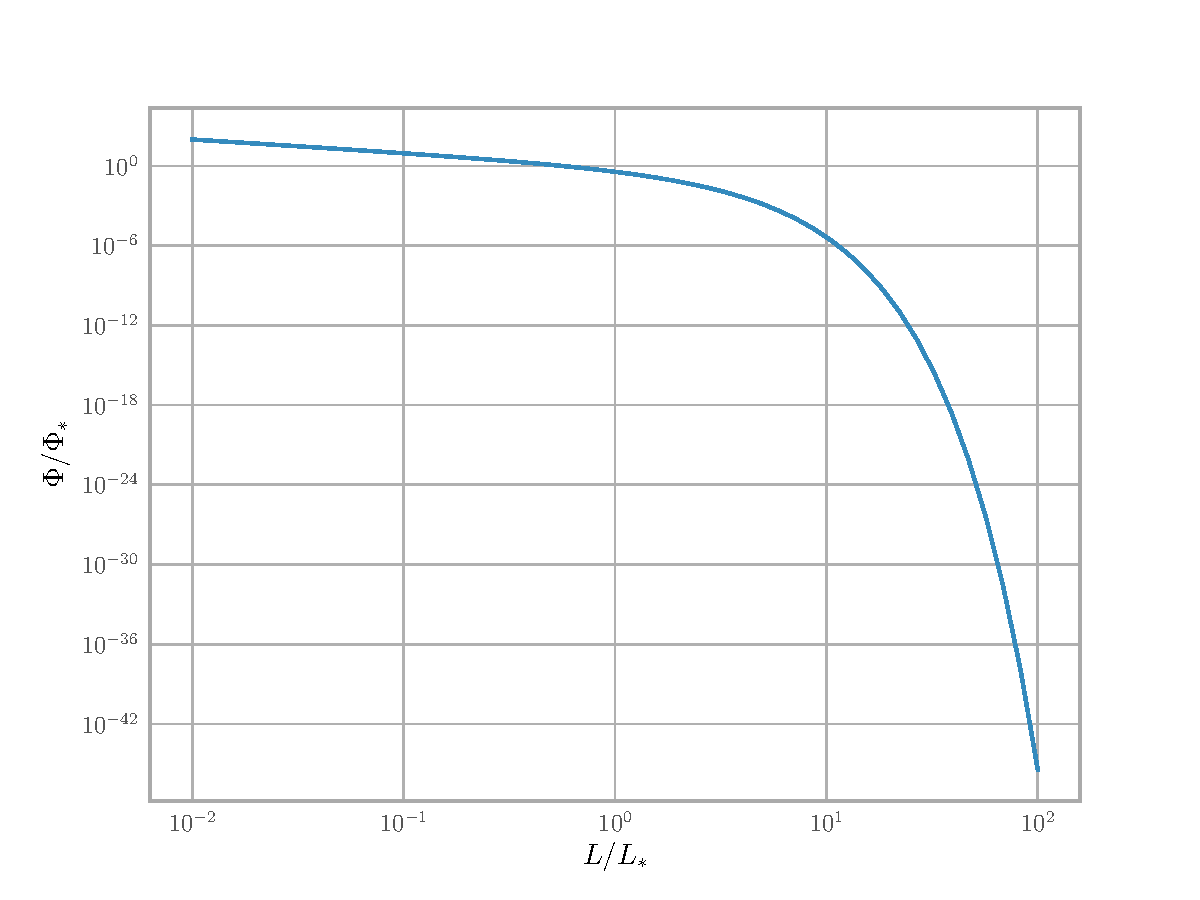
\includegraphics[width=\textwidth]{figures/Schechter.pdf}
\caption{A rough plot of the Schechter function for \(\alpha = 1\).}
\label{fig:Schechter}
\end{figure}

The integral for \(\mathscr L_g\) converges despite the divergence of \(\Phi(L)\) as \(L \rightarrow 0\), since it is multiplied by \(L\): so we do not need to really worry about the low-luminosity divergence of the distribution.

The result of the integral for a generic value of \(\alpha \) is \(\mathscr L_g = \Phi^* L^* \Gamma(2-\alpha)\), where \(\Gamma\) is the Euler gamma function; for the \(\alpha = 1\) case we get a factor \(\Gamma(2-1) = 1\).

Numerically, we get \(\mathscr{L}_{g} \approx \num{e8} h L_\odot \SI{}{\per\cubic\mega\parsec}. \) 
\todo[inline]{This is reported incorrectly in \cite{Pacciani:2018} as \(\sim \num{e18}\)! The correct figure can be found in \cite[eq. 4.5.14]{LucchinColes:2002}.
I do not think there is much of a point in reporting the specific value, since the parameters are already given as order-of-magnitude estimates.}

Now, we must estimate \(\expval{M / L}\).
The luminosity of galaxies can be measured readily, the great difficulty lies in estimating their mass.

\subsection{Estimating the masses of galaxies}

We must distinguish between the different shapes of the galaxies:

Spiral galaxies are characterized by rotation.

We plot the velocity of rotation of galaxies \(v\)  against the radius \(R\). This is measured using the Doppler effect.

We'd expect a roughly linear region, and then a region with \(v \sim R^{-1/2}\):
we apply \(G M(R) = v^2 (R) R\) (this comes from Kepler's laws or from the virial theorem). This implies

\begin{equation}
  v(R) \propto \sqrt{\frac{M(R)}{R}}
\end{equation}

So in the inside of the galaxy, where \(M(R) \propto R^3\), \(v \propto R\), while outside of it \(M(R)\) is roughly constant, so \(v \propto R^{-1/2}\).

Instead of this, we see the linear region and then \(v(R)\) is approximately constant. Is Newtonian gravity wrong? (GR effects are trivial at these scales).

An option is MOND: they propose that there is somthing like a Yukawa term at Megaparsec distances. They are wrong for some other reasons.

Another option is that what we thought was the galaxy, from our EM observations, is actually smaller than the real galaxy. We'd need mass obeying \(M (R) \sim R\): since \(M(R) = 4 \pi \int_0^{R_{\text{max}}} \dd{R} R^2 \rho(R)\), we need \(\rho(R) \propto R^{-2}\). This is a \emph{thermal} distribution (?): we call it the \emph{dark matter halo}.

People tend to believe that this matter is made up of beyond-the-standard-model particles, like a \emph{neutralino}.
An alternative is the \emph{axion}.

The total density of DM is \(\sim 5\) times more than that of regular matter.

If galaxies are not spiral, we look at other things: the Doppler broadening of spectral lines gives us a measure of the RMS velocity.

\subsection{Virial theorem}

Later in the course we will obtain the (nonrelativistic) virial theorem:

\begin{equation}
  2T + U = 0
\end{equation}

This holds when the inertia tensor stabilizes.

The kinetic energy is \(T = \frac[i]{3}{2} M \expval{v_r^2} \): we expect the radial velocity to account for one third of total energy by equipartition.
\(M\) is the total mass of the energy.

The potential energy is \(U = - G M^2 /R\). Substituting this in we get \(3 \expval{v_r^2} = GM/R\).

If we account for the extra DM mass, we get \(\expval{M/L} \approx 300 h M_\odot / L_\odot\).
In order to have \(\Omega = 1\), we'd need 1390.

So measuring the number density of galaxies and their velocities we get a way to measure \(\Omega_0\).

So, only \(5\%\) of the energy budget is given by baryionic matter (not all of which is visible), while around \(27\%\) is dark matter.

In order to comply with observation, it must be:

\begin{equation}
  0.013 \leq \Omega_{\text{b}} h^2 \leq 0.025\,,
\end{equation}
%
where \(\Omega_b\) corresponds to the baryionic density: so the universe \emph{cannot} be made only of baryons.

Dark matter likes ``clumping'': we characterize it by this property.

In the end we have \(\Omega = 1 = \Omega_b + \Omega_{DM} + \Omega_{DE}\) (do note that the value of 1 is measured, not theoretical!)

The Friedmann equation would imply deceleration if \(\rho, P \geq 0\): dark energy seems to have \emph{negative pressure}.

What about radiation? The CMB appears to be Planckian:

\begin{equation}
  \rho_{0 \gamma} = \frac{\sigma_r T_{0 \gamma}^4}{c^2} = \SI{4.8e-34}{\gram\per\centi\metre\cubed}
\end{equation}
%
where \(\sigma_r = \pi^2 k_B^4 / (15 \hbar ^3 c^3)\), while \(\sigma_{SB} = \sigma_r c /4\).

We are going to show that if neutrinos were massless, their temperature would be \(T_\nu = (4/11)^{1/3} T_\gamma\).

However, we know that for sure \(\sum m_\nu \leq \SI{0.12}{eV} \).

We have:
%
\begin{equation}
  \rho_\nu = 3 N_\nu \frac{\expval{m_\nu} }{\SI{10}{eV}} \SI{e-30}{\gram\per\cubic\centi\metre}
\end{equation}
(??? to check)

\subsection{The Hubble law}

It is very simply

\begin{equation}
  v = H_0 d\,,
\end{equation}
%
where \(v\) is the velocity of objects far from us, and \(d\) is their distance from us. Can we derive this from the Robertson-Walker line element?
It was actually derived first by Lemaitre.

We drop the angular part in the FLRW line element (for \(k = 0\)):

\begin{equation}
  \dd{s^2} = c^2 \dd{t^2} - a^2(t) \dd{r^2}
\end{equation}

So the distance \(d = a(t) r\): therefore \(\dot{d} = \dot{a}r = \frac{\dot{a} }{a} d\).   This is Newtonian and rough, but it seems to work.

\begin{definition}[Redshift]
    The redshift \(z\) is defined by
    %
    \begin{equation}
      z = \frac{\lambda_0 - \lambda_e}{\lambda_{e}}\,,
    \end{equation}
    %
    where \(\lambda_0\) and \(\lambda_e\) are the observed and emission wavelengths.
\end{definition}

We can show that \(1+z = a_0/ a_e\). Therefore, \(\nu_o / \nu_e = a_e / a_0\).

So, we can define (?) the luminosity distance:
%
\begin{equation}
  d_L = \sqrt{\frac{L}{4 \pi \ell} } \,,
\end{equation}
%
where \(L\) is the observed luminosity, while \(\ell\) is the apparent luminosity.

How do we relate the luminosity distance and the scale factor? Geometrically we derive:
%
\begin{equation}
  \ell = \frac{L}{4 \pi r^2 a^2} \qty(\frac{a_e}{a_0}) ^2
\end{equation}
%
since we can just integrate over angles the FLRW element: the value of \(k\) does not enter into the equation.
The corrective factor comes from the frequency dependence of energy and the fact that power is energy over time, which also changes.

Therefore:
%
\begin{equation}
  d_L = \frac{a_o^2}{a_e} r = a (1+z) r\,.
\end{equation}


\end{document}
